\documentclass[12pt,letterpaper]{article}
\usepackage[utf8]{inputenc}
\usepackage[spanish, es-tabla]{babel}
\usepackage[version=3]{mhchem}
\usepackage[journal=jacs]{chemstyle}
\usepackage{amsmath}
\usepackage{amsfonts}
\usepackage{amssymb}
\usepackage{makeidx}
\usepackage{xcolor}
\usepackage[stable]{footmisc}
\usepackage[section]{placeins}
\usepackage{array}
\usepackage{xtab}
\usepackage{multirow}
\usepackage{colortab}

\sisetup{mode=text, output-decimal-marker = {,}, per-mode = symbol, qualifier-mode = phrase, qualifier-phrase = { de }, list-units = brackets, range-units = brackets, range-phrase = --}

\usepackage{cancel}
%Paquetes necesarios para imágenes, pies de página, etc.
\usepackage{graphicx}
\usepackage{lmodern}
\usepackage{fancyhdr}
\usepackage[left=4cm,right=2cm,top=3cm,bottom=3cm]{geometry}

%Instrucción para evitar la indentación
%\setlength\parindent{0pt}
%Paquete para incluir la bibliografía
\usepackage[backend=bibtex,style=chem-acs,biblabel=dot]{biblatex}
\addbibresource{references.bib}

%Formato del título de las secciones

\usepackage{titlesec}
\usepackage{enumitem}
\titleformat*{\section}{\bfseries\large}
\titleformat*{\subsection}{\bfseries\normalsize}

%Creación del ambiente anexos
\usepackage{float}
\floatstyle{plaintop}
\newfloat{anexo}{thp}{anx}
\floatname{anexo}{Anexo}
\restylefloat{anexo}
\restylefloat{figure}

%Modificación del formato de los captions
\usepackage[margin=10pt,labelfont=bf]{caption}

%Paquete para incluir comentarios
\usepackage{todonotes}

%Paquete para incluir hipervínculos
\usepackage[colorlinks=true, 
            linkcolor = blue,
            urlcolor  = blue,
            citecolor = black,
            anchorcolor = blue]{hyperref}

%%%%%%%%%%%%%%%%%%%%%%
%Inicio del documento%
%%%%%%%%%%%%%%%%%%%%%%

\begin{document}
\renewcommand{\labelitemi}{$\checkmark$}

\renewcommand{\CancelColor}{\color{red}}

\newcolumntype{L}[1]{>{\raggedright\let\newline\\\arraybackslash}m{#1}}

\newcolumntype{C}[1]{>{\centering\let\newline\\\arraybackslash}m{#1}}

\newcolumntype{R}[1]{>{\raggedleft\let\newline\\\arraybackslash}m{#1}}

\begin{center}
	\textbf{\LARGE{Cloud Computing}}\\
	\vspace{4mm}
	\textbf{\large{Luis Aseguinolaza, Tom\'as Pitinari, Manuel Uliassi}}\\
	\vspace{4mm}
	\textbf{\large{Profesor: Alejandro Rodriguez Costello}}\\
\end{center}

\vspace{7mm}

\section*{\centering Introducci\'on}

Es un paradigma que permite ofrecer servicios de computación a través de una red, que usualmente es Internet.
Cloud computing es un nuevo modelo de prestación de servicios de negocio y tecnología, que permite incluso al usuario acceder a un catálogo de servicios estandarizados y responder con ellos a las necesidades de su negocio, de forma flexible y adaptativa, en caso de demandas no previsibles o de picos de trabajo, pagando únicamente  por el consumo efectuado, o incluso gratuitamente en caso de proveedores que se financian mediante publicidad o de organizaciones sin ánimo de lucro.


\section{Tipos de Servicios}

El cambio que ofrece la computación desde la nube es que permite aumentar el número de servicios basados en la red. Esto genera beneficios tanto para los proveedores, que pueden ofrecer, de forma más rápida y eficiente, un mayor número de servicios, como para los usuarios que tienen la posibilidad de acceder a ellos, disfrutando de la ‘transparencia’ e inmediatez del sistema y de un modelo de pago por consumo. Así mismo, el consumidor ahorra los costes salariales o los costes en inversión económica (locales, material especializado, etc.).

El concepto de “nube informática” es muy amplio, y abarca casi todos los posibles tipo de servicio en línea, pero cuando las empresas predican ofrecer un utilitario alojado en la nube, por lo general se refieren a alguna de estas tres modalidades:
\begin{enumerate}
\item Saas (Software as a Service):Ofrecen una aplicación en la nube como servicio. Ejemplos: Gmail, Office 365, Outlook, etc.
\item Paas (Platform as a service): Ofrece un entorno como servicio, pensado principalmente para desarrolladores. Ejemplos: Red hat OpenShift, Google App Engine.
\item Iaas (Infraestructure as a service): Ofrecen infraestructuras de almacenamiento y máquinas virtuales en la nube. Ejemplos: Azure, Amazon Web Services, vCloud, Openstack.
\end{enumerate}

\subsection{Caracteristicas:}
\begin{itemize}
\item Agilidad.
\item Costos menores que una instalacion fisica.
\item Escalabilidad y elasticidad.
\item Independencia entre dispositivo y ubicacion.
\item La virtualizacion permite compartir servidores y dispositivos de almacenamiento. Las aplicaciones pueden ser facilmente migradas de un servidor fisico a otro.
\item Los sistemas en la nube optimizan los recursos utilizados de manera automatica.
\item Es mas seguro que los datos alojados en el servidor esten centralizados, ya que el usuario es responsable de la seguridad de la aplicacion, mientras que el proveedor es responsable de la seguridad fisica.
\item El mantenimiento se vuelve mas sencillo, ya que la aplicacion no necesita estar en el ordenador del usuario, y puede accederse desde diferentes lugares.
\end{itemize}

\subsection{Ventajas:}

\begin{itemize}
\item La integracion de las aplicaciones es mucho mas facil y sencillo.
\item Poseen una gran distribucion de infraestructuras a nivel mundial.
\item Una infraestructura 100 \% de cloud computing permite también al proveedor de contenidos o servicios en la nube prescindir de instalar cualquier tipo de software, ya que este es provisto por el proveedor de la infraestructura.
\item Implementación más rápida y con menos riesgos, ya que se comienza a trabajar más rápido y no es necesaria una gran inversión.
\item Actualizaciones automaticas sin la necesidad de que el usuario gaste tiempo y recursos en hacerlo por si mismo.
\item Tienen un consumo eficiente de energia, ya que usan solo la necesaria.
\end{itemize}

\subsection{Desventajas:}
\begin{itemize}
\item La centralización de las aplicaciones y el almacenamiento de los datos origina una interdependencia de los proveedores de servicios.
\item La disponibilidad de las aplicaciones está sujeta a la disponibilidad de acceso a Internet.
\item La confiabilidad de los servicios depende de la "salud" tecnológica y financiera de los proveedores de servicios en nube.
\item La disponibilidad de los servicios altamente especializados podrian tardar mucho hasta ser desplegados en al red.
\item La modificacion constante de las interfaces debido a la madurez funcional de las aplicaciones hace  que la curva de aprendizaje de las empresas nos tecnologicas tengan una pendiente significativa.
\item La seguridad de la informacion, ya que debe recorrer diferentes modos para llegar a su destino. Si se utilizan encriptaciones para proteger estos datos, la velocidad de estos disminuye debido a la sobrecarga que estos encriptamientos significa.
\item Escalabilidad a largo plazo, esto quiere decir que cuando el servicio tenga mayor demanda, la empresa debera tener un plan de expansion para que sus servicios no se deterioren.
	\end{itemize}	
	
\subsection{Tipos de Nubes:}
	\begin{enumerate}

\item Una nube publica es mantenida y gestionada por terceros no vinculados con la organizacion. En este tipo de nubes tanto los datos como los procesos de varios clientes se mezclan en los servidores, sistemas de almacenamiento y otras infraestructuras de la nuble. Los usuarios no conocen los trabajos que los otros clientes corren en el servidor.
\item Las nubes privadas son una buena opción para las compañías que necesitan alta protección de datos y ediciones a nivel de servicio. Las nubes privadas están en una infraestructura bajo demanda, gestionada para un solo cliente que controla qué aplicaciones debe ejecutarse y dónde. Son propietarios del servidor, red, y disco y pueden decidir qué usuarios están autorizados a utilizar la infraestructura.
\item Las nubes híbridas combinan los modelos de nubes públicas y privadas. Un usuario es propietario de unas partes y comparte otras, aunque de una manera controlada. Un ejemplo son los sistemas de correo electrónico empresarial.
		\end{enumerate}	
		
		
\section {OpenStack:}
Es una plataforma Cloud Computing de software libre y código abierto. Está 
diseñada para ofrecer nubes públicas o privadas orientadas a brindar infraestructuras
 como servicio a los usuarios (Iaas) y para poder desplegar máquinas virtuales. 
Más de 200 empresas se unieron al proyecto entre las que destacan AMD, Cisco, Dell,
 Ericsson, HP, IBM, Intel, Yahoo!, etc.
Su tecnología consiste en una serie de proyectos relacionados entre sí que controlan
 procesamiento, almacenamiento y recursos de red a través de un centro de datos, todos
 administrados a través de un panel de control que permite a los administradores 
controlar mientras potencia a sus usuarios proveyendo los recursos a través de una 
interfaz web.

\subsection{Sus componentes:}
    \begin{enumerate}
    \item  Ceilometer: Este componente nos brinda la capacidad de poder ajustar y transformar datos en los 
componentes de OpenStack para que se adapten a ellos, se utiliza para poder controlar
los distintos usuarios debido a sus tres principales funciones, estas son "Metering",
recopila información con respecto a cualquier cosa que se pueda facturar y devuelve
el resultado en un conjunto de "tickets", "Rating", analiza un conjunto de tickets
para tranformarlo en un "bill line item", y "Billing", proceso que ensambla todos los
"bill line item" y devuelve una sola factura por cliente.

\item  Cinder:
es el servicio de almacenamiento en bloque de OpenStack para proporcionar volúmenes. 
Nos facilitará acceso al contenido alojado en las unidades de disco que se encuentren 
en nuestra cloud. Sus principales ventajas son que se pueden añadir rápidamente nuevos 
comportamientos, que las fallas son fáciles de diagnosticar, depurar y rectificar y que
los procesos aislados evitan fallos en cascada.
\item  Glance:
Con Glance dispondremos de un servicio de gestión de imágenes (copias íntegras de las
 unidades de disco duro de las que dispongamos).
\item  Heat:
Heat nos permitirá establecer los requisitos de una aplicación que sirvamos desde 
nuestra nube, en un archivo que define los recursos necesarios para dicha aplicación. 
\item  Horizon:
El que se encarga de mostrarnos mediante una interfaz gráfica toda la gestión de 
OpenStack , desde donde podremos ver qué está pasando en nuestra nube y gestionarla.
\item  Keystone:
Este servicio controlará la identificación de los diferentes usuarios que se conecten
 a nuestra infraestructura, y el acceso a según qué servicios o aplicaciones de los 
mismos.
\item  Neutron:
Que cada módulo de OpenStack se comunique con otro y estén interrelacionados , es 
gracias a Neutron, que se encarga de que cada componente desplegado en OpenStack.
\item  Nova:
Considerado el “motor” de OpenStack. Es usado para desplegar y administrar la cantidad
 de máquinas virtuales y otros servicios que necesitemos .
\item  Swift:
Se trata del módulo encargado de almacenar los archivos del sistema, asegurar su 
integridad y replicarlos por los diferentes discos que encontramos en la 
infraestructura, para que éstos siempre estén disponibles y accesibles de la forma más
 rápida posible.
	\end{enumerate}	
		
\section {Chef:}
Chef es un software basado en Ruby diseñado para mantener y configurar servidores. Se puede integrar junto con Openstack para generar y configurar nuevas máquinas virtuales.
\\Una nube con Chef se compone por: 
\begin{enumerate}
\item Chef Server: gestiona los nodos que componen la infraestructura.
\item Chef Client: es un programa que corre en cada nodo, se encarga de comunicarse con el Chef Server. Cada vez que un Nodo quiere utilizar una Estación de Trabajo, se fija si hay cambios en la Estación. De haberlos, el Chef Server le envía al cliente los cambios, y luego el cliente los guarda. Luego de haber obtenido los últimos cambios, el Nodo envía los suyos.
\item Nodos: son los usuarios finales.
\item Estaciones de Trabajo: son las maquinas que proveen de poder de computo.
\end{enumerate}

\begin{figure}[h]
\centering
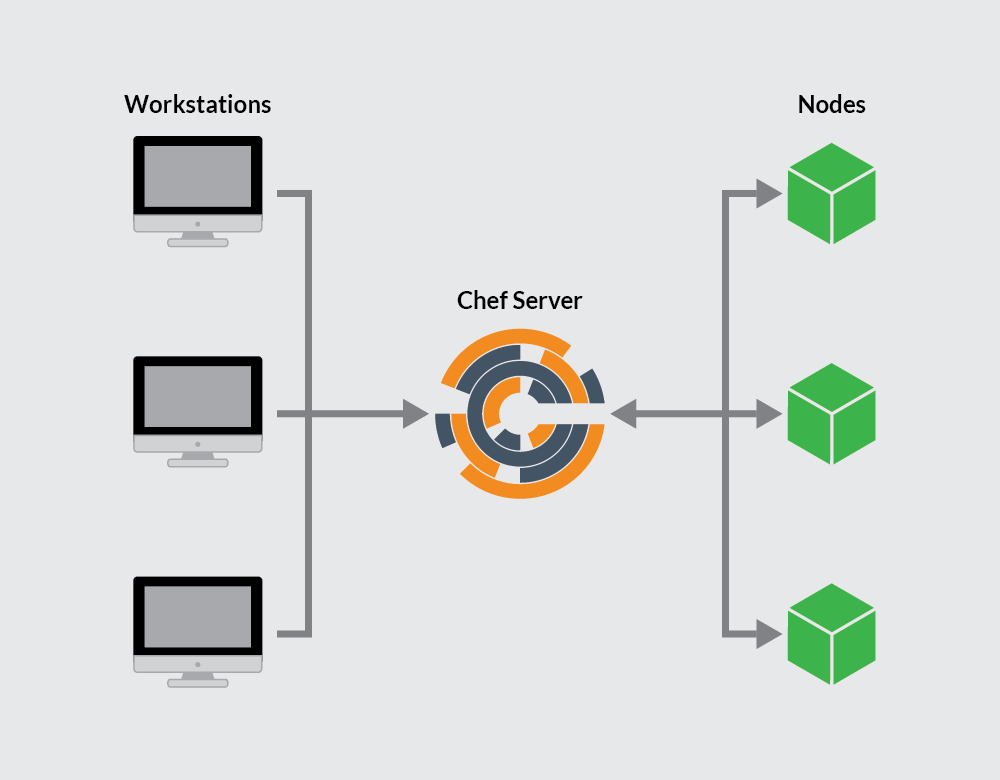
\includegraphics[width=1\textwidth]{chef-graph.png}
\end{figure}

\subsection{Recetas:}
El administrador escribe recetas, que describen como Chef debe manejar las aplicaciones del servidor. Al conjunto de recetas se lo denomina libro de cocina (Cookbook). Dentro de las recetas se especifica en qué estado deben estar los recursos: Que paquetes deben estar instalados, que servicios deben estar en ejecución, y que archivos deban ser escritos. Estos recursos pueden ser configurados para versiones específicas de software, y se puede asegurar que ese software este correctamente instalado, teniendo en cuenta sus dependencias.

\subsection{Escalabilidad:}
Chef, además cuenta con manejo automático de configuración, para mantener infraestructuras a gran escala. La infraestructura se define como código, asegurando que la configuración sea flexible, versionable y testeable. Los servidores que maneja Chef están continuamente siendo comparados y corregidos con el estado en el que deberían estar. 

\end{document}

